\section{Bipartite Graphs}
We've mentioned bipartite graphs several times in different chapters of this book. However, we've only explored this class of graph at a surface level. In this section, we'll take a deeper look into bipartite graph - what are the conditions for being bipartite, how do bipartite graphs allow us to more easily answer certain questions, and how are they relevant in our own real scenarios?

\subsection{Definitions}
Let's give a formal definition for what it means for a graph to be bipartite. First, let's define what an independent vertex set is:

\begin{definition}[Independent Vertex Set]
    An \textit{independent vertex set} is a set of vertices in a graph $G$, none of which are adjacent.
\end{definition}

Using this, we can give a good definition for bipartite graphs:

\begin{definition}[Bipartite Graph]
    A graph $G$ is \textit{bipartite} if its vertex set can be partitioned into two independent vertex sets.
\end{definition}

This is no different than how we've defined them before. Here are some examples of bipartite graphs:

\begin{center}
    \begin{tabular}{c c}
        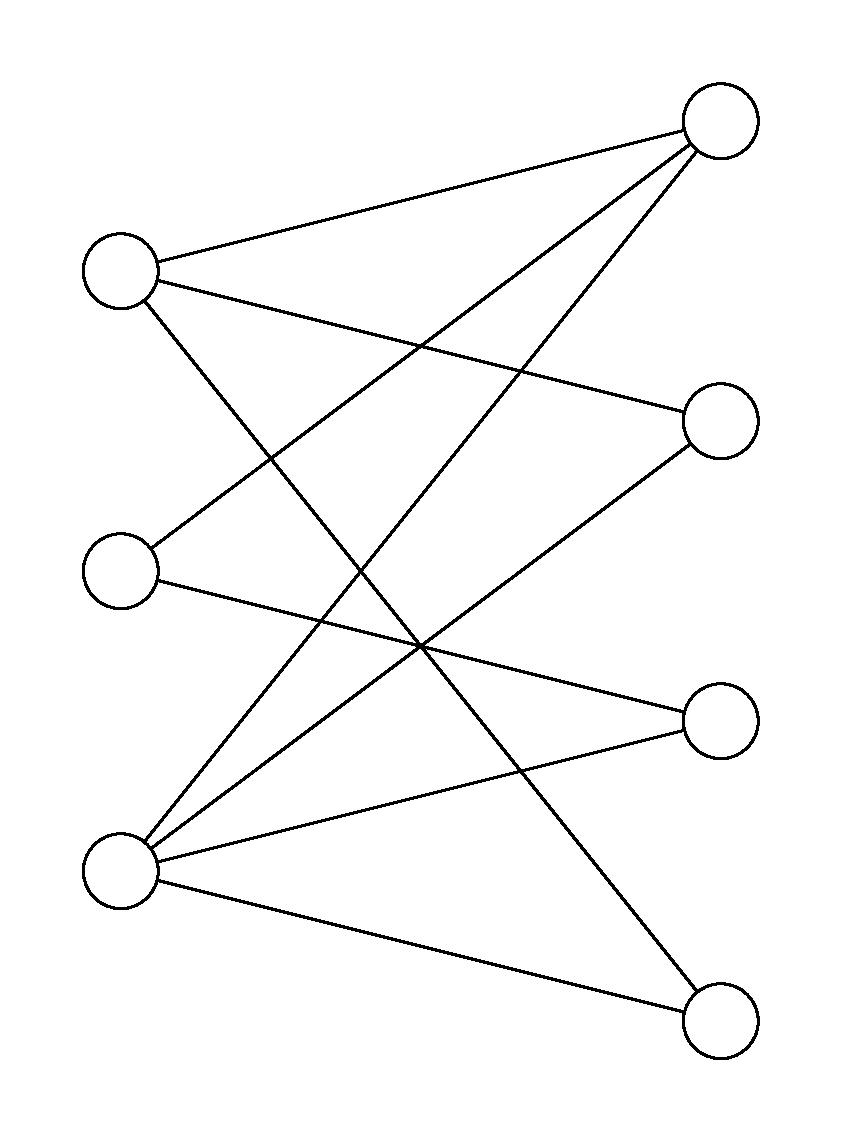
\includegraphics[width=0.3\textwidth]{Project3/Bipartite/bip.pdf} & 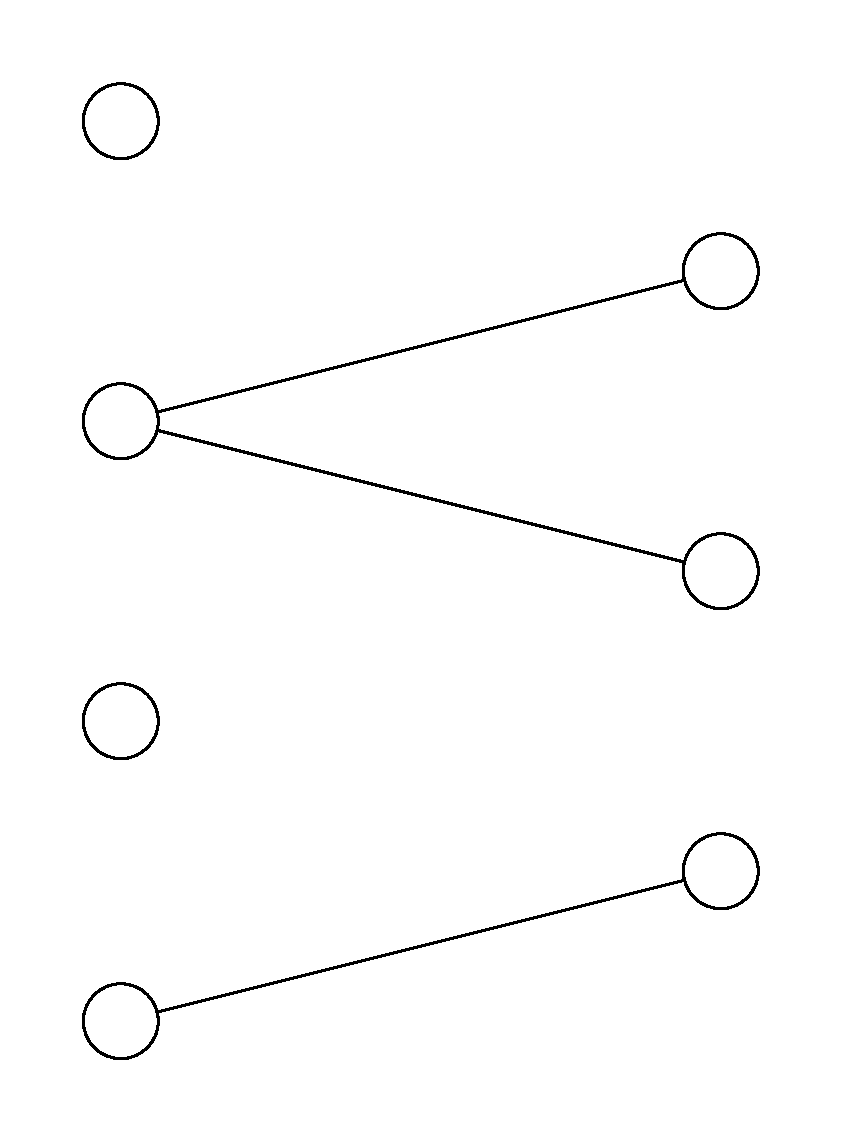
\includegraphics[width=0.3\textwidth]{Project3/Bipartite/forest.pdf} \\
        Connected Bipartite Graph & Disconnected Bipartite Graph
    \end{tabular}
\end{center}

Having defined bipartite, we can derive several other related classes of graphs, including complete bipartite, or tripartite. There are other classes as well which are equivalent to or are subsets of the set of bipartite graphs. For example, all trees are bipartite (this is easy to imagine, and there are some different proof strategies for this). Cycles of even length are bipartite as well, though cycles of odd length are not. 

Complete bipartite graphs are an important subset of bipartite graphs. Here is the formal definition for complete bipartite:

\begin{definition}[Complete Bipartite Graph]
    A \textit{complete bipartite} graph $G$ is a graph whose vertex set can be partitioned into two independent sets $U$ and $V$ such that for any $u \in U$ and $v \in V$, $(u, v)$ is an edge. Such a graph is denoted as \[ K_{m,n} \] where $m, n$ are the sizes of each independent set.
\end{definition}

An example of a complete bipartite graph is $K_{3,3}$, known as the Utility Graph, shown below:

\begin{center}
    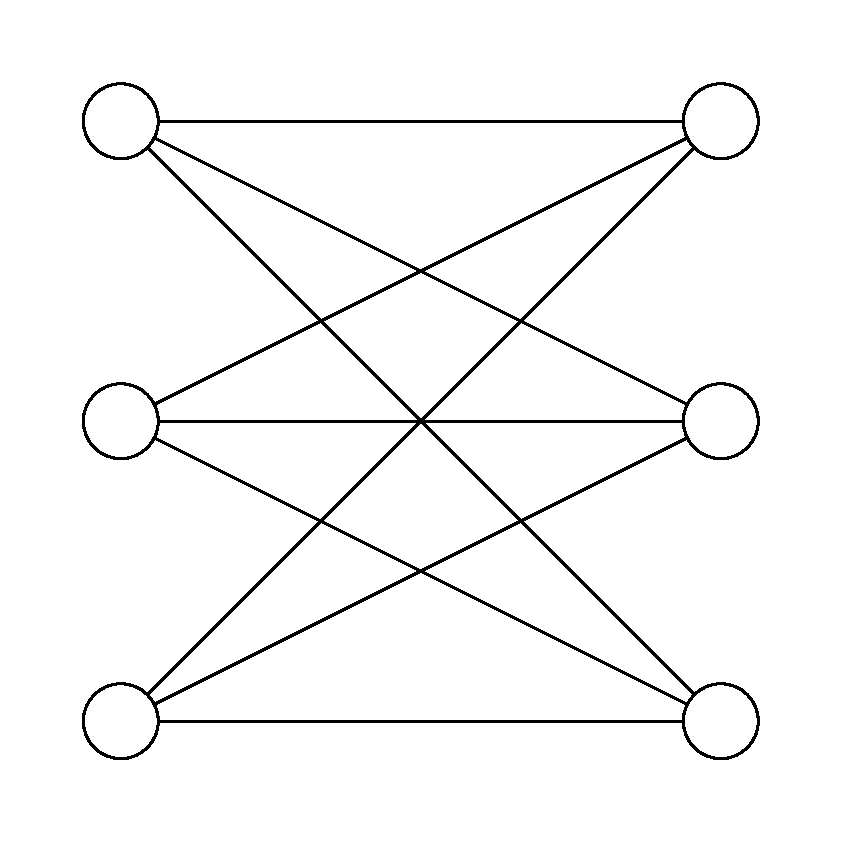
\includegraphics[width=0.4\textwidth]{Project3/Bipartite/k33.pdf}
\end{center}

\subsection{When Can We Use These?}
As you might imagine, bipartite graphs might be useful when we want to take information in two distinct categories, and match them. For example, suppose we want to consider the relationships between professors and courses they teach. In our graph, we can separate these into two categories, "professors" and "courses", and create an edge any time a particular professor teaches a course. By construction, we have that there would not be any edges between two professors (as a professor is not a course), nor would there be any edges between two courses (as a course cannot teach another course). Thus, we have a bipartite relationship by construction.

\begin{center}
    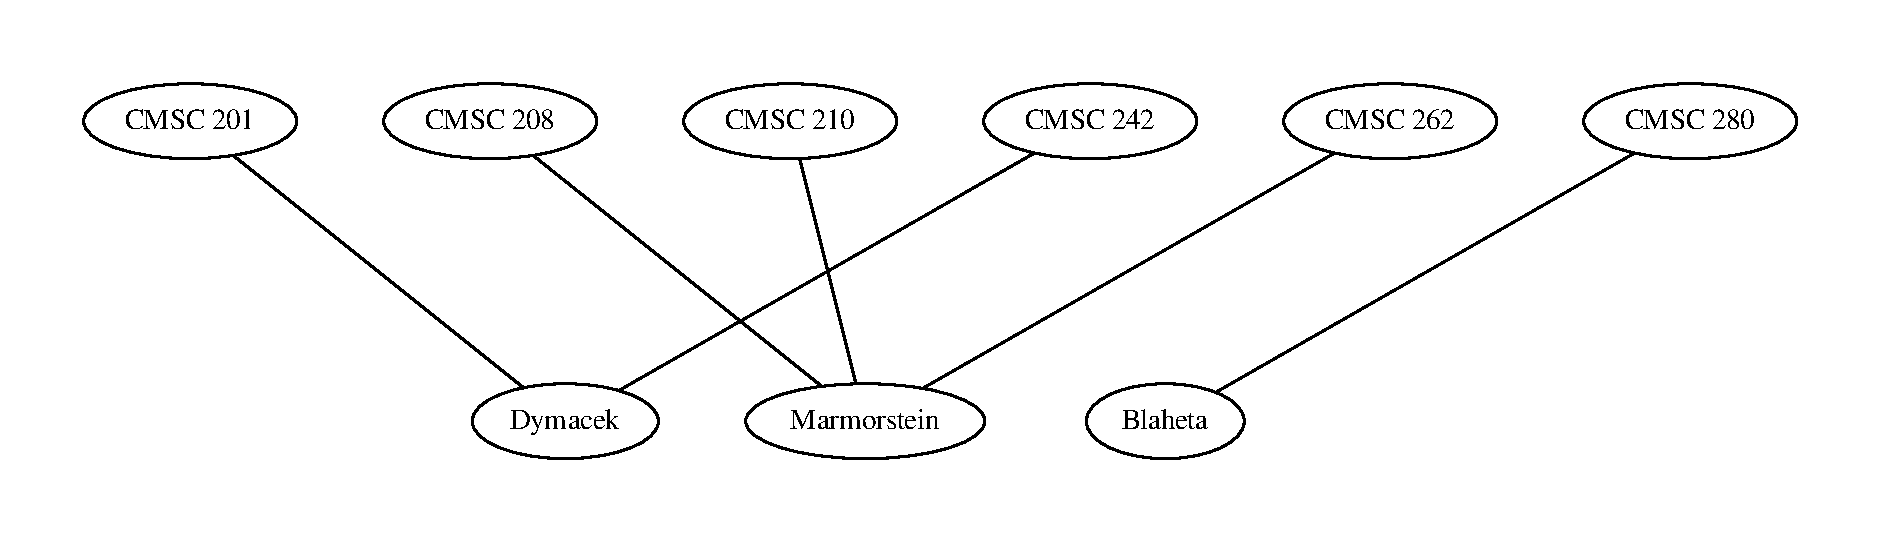
\includegraphics[width=\textwidth]{Project3/Bipartite/boxed.pdf}
\end{center}

A classical example of this problem is something we've covered before - the Knight's Tour. On a chessboard, the movement pattern of a knight allows us to separate the spaces on a chessboard into sets of light and dark spaces. When the knight moves, the space it lands on alternates color. Drawing edges between a particular space and all other spaces to which the knight can move, we construct a bipartite graph!

\subsection{How Does This Help Us?}
Given a bipartite graph, it becomes much easier to determine asnwers to certain historically difficult problems. For example, if $G$ is bipartite with an odd number of vertices, then we know for certain that $G$ is non-hamiltonian. This was proven in previous exercises, and can easily be found online. 

Regarding cliques, we know that if $G$ is bipartite, then its clique number is 2. If $G$ has a clique number $c > 2$, then we could find a complete subgraph of size $c$, which would contain a triangle. However, to be bipartite, we cannot have a triangle, and thus $G$ would not be bipartite. 

Finally, regarding graph coloring, if $G$ is a bipartite graph, then we know that the chromatic number of $G$ is 2. We can achieve this by coloring each independent set one color (since no vertices in either set are adjacent to each other). Thus we have two colors covering all vertices, so $\chi(G) = 2$.
